% !TeX spellcheck = cs_CZ
% Lineární obvody a systémy - Jan Bičák  - strana 10
% Popis spojitých systémů
%===================================================================================================
\begin{example}Lineární spojitý systém je dán zapojením dle obrázku. Určete:
  \begin{enumerate}
    \item diferenciální rovnici pro odezvu $u_2(t)$, je-li na vstupu buzen napětím $u_1(t)$,
    \item přenos napětí $H(p)=\dfrac{U_2(p)}{U_1(p)}$,
    \item impulsní odezvu $h(t)$.
  \end{enumerate}

   {\centering
    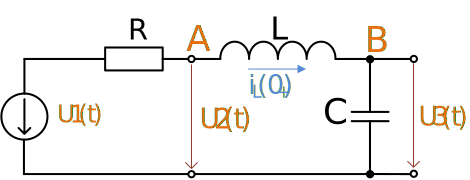
\includegraphics[scale=0.5]{cir_RLC.pdf}
    \captionof{figure}{Zapojení obvodu RLC.}
    \label{SAS:fig_RLC}
    \par}
  \textbf{Řešení:}\newline
  Pro zapojení dle obrázku získáme metodou uzlových napětí integrodiferenciální rov\-ni\-ce pro
  uzly \texttt{A} a \texttt{B}:
  \begin{align}\label{SAS:eq_RLC_basic_rces}
    A &:  \frac{u_3(t)-u_1(t)}{R}+\frac{1}{L}
    \int_0^t{(u_3(t)-u_2(t))}d\tau+i_L(0_+) = 0\,               \\ \nonumber
    B &:  \frac{1}{L}\int_0^t{(u_2(t)-u_3(t))}d\tau+C\frac{du_c}{dt}-i_L(0_+)        = 0
  \end{align}
  Derivováním a eliminací $u_3(t)$ z původních rovnic dostaneme pro odezvu $u_2(t)$ diferenciální
  rovnici II. řádu
  \begin{itemize}
    \item \(\frac{d}{dt}(B)\):
          \begin{equation*}
            u_2(t)-u_3(t)+LC\frac{d^2u_2(t)}{dt^2}
            =0\Rightarrow u_3(t)=u_2 (t)+LC\frac{d^2u_2(t)}{dt^2}
          \end{equation*}
    \item \(\frac{d}{dt}(B)\rightarrow(A)\):
  \end{itemize}
  \begin{align*}
    \frac{u_2(t)+LC\frac{d^2u_2(t)}{dt^2}-u_1(t)}{R}+
    \frac{1}{L}\int_0^t{(LC\frac{d^2u_2(t)}{dt^2})}d\tau+i_L(0_+) &=  0 \\
    u_2(t)+LC\frac{d^2u_2(t)}{dt^2}-u_1(t)+
    RC\left[\frac{du_2(t)}{dt}\right]_0^t+Ri_L(0_+)               &=  0
  \end{align*}
  Při nulových počátečních podmínkách: $\frac{du_2(t)}{dt}|_{t=0}=0$, $i_L(0_+)=0$ dostaneme:
  \begin{equation}\label{sas:eq_dif_RLC_II_r}
    LC\frac{d^2u_2(t)}{dt^2}+RC\frac{du_2(t)}{dt}+u_2(t)=u_1(t)
  \end{equation}
  V Laplaceově transformaci platí:
  \begin{align*}
    \mathcal{L}\left[\frac{du_2(t)}{dt}\right]     &= pU_2(p)-u_2(0) \\
    \mathcal{L}\left[\frac{d^2u_2(t)}{dt^2}\right] &= p^2U_2(p)-pu_2(0)-u_2(0),\,kde\,u_2(0)=
    \frac{du_2(t)}{dt}|_{t=0}
  \end{align*}
  při nulových počátečních podmínkách
  \begin{equation}\label{sas:eq_L_RLC_rce}
    p^2LCU_2(p)+pRCU_2(p)+U_2(p)=U_1(p)
  \end{equation}
  Odtud vyplývá \textbf{přenosová funkce} $H(p)=\frac{U_2(p)}{U_1(p)}$
  \begin{equation}\label{sas:eq_Hp_RLC}
    H(p)=\frac{1}{p^2LC+pRC+1}
        =\frac{1}{LC}\frac{1}{p^2+p\frac{R}{L}+\frac{1}{LC}}=\frac{Q(p)}{N(p)}
  \end{equation}
  K nalezení \textbf{impulsní odezvy} nejprve určíme póly přenosové funkce řešením rovnice
  $N(p)=0$
  \begin{equation}\label{sas:eq_koreny_L_rce}
    p_{\infty_{12}}=\frac{\frac{R}{L}\pm\sqrt{\left(\frac{R}{L}\right)^2-\frac{4}{LC}}}{2}
    =\frac{R}{2L}\pm\sqrt{\left(\frac{R}{2L}\right)^2-\frac{1}{LC}}
  \end{equation}
  přenosovou funkci pak upravíme do tvaru
  \begin{equation}\label{sas:eq_Hp_forma}
    H(p)=\frac{K}{(p-p_{\infty_1})\cdot(p-p_{\infty_2})}, \qquad K=\frac{1}{LC}
  \end{equation}
  \begin{itemize}
    \item Uvažujeme-li jednoduché póly a bude-li $R>2\sqrt{\frac{L}{C}}$ , potom z  rov.
          \ref{sas:eq_koreny_L_rce} vyplývají dva reálné různé póly. Přenosovou funkci tedy můžeme
          zapsat obecným tvarem:
          \begin{equation}\label{sas:eq_Hp_forma_2}
            H(p)=\frac{K}{(p+a_1)\cdot(p+a_2)}=\frac{k_1}{p+a_1}+\frac{k_2}{p+a_2}
          \end{equation}
          kde $p_{\infty_1}=-a_1,\, p_{\infty_2}=-a_2$, Rezidua  $k_1=\frac{K}{a_2-a_1}$,
          $k_2=\frac{K}{a_1-a_2}$ určíme z rov. \ref{sas:eq_HP_rezidua}. Impulsní odezvu pak
          vypočteme užitím rov. \ref{sas:eq_impulzni_odezva}.
          \begin{equation}\label{sas:eq_ht1}
            h(t)=\mathcal{L}^{-1}[H(p)]=\frac{K}{a_2-a_1}e^{-a_1t}+\frac{K}{a_1-a_2}e^{-a_2t}
          \end{equation}
    \item Když bude $R<2\sqrt{\frac{L}{C}}$, obdržíme dvojici komplexně sdružených pólů a
          pře\-no\-so\-vou funkci může obecně zapsat takto:
          \begin{equation}\label{sas:eq_ht2}
            H(p)=\frac{K}{(p+a_1)\cdot(p+a_2)}=\frac{k_1}{p+a-jb}+\frac{k_2}{p+a+jb}
          \end{equation}
          kde $p_{\infty_1}=-a+jb$, $p_{\infty_2}=-a-jb$. Rezidua v pólech jsou dány výrazy
          $k_1=-\frac{jK}{2b}$, $k_2=\frac{jK}{2b}$. Impulzní odezvu opět určíme užitím rov.
          \ref{sas:eq_impulzni_odezva}.
          \begin{equation*}
            h(t) = \frac{Ke^{-at}}{2b}\left[j\cdot\left(-e^{jbt}+e^{-jbt}\right)\right]
          \end{equation*}
          \begin{align}
            \,  &= \frac{Ke^{-at}}{2b}\left[j\cdot
            \left(\underline{-\cos(bt)}-j\sin(bt)+
            \underline{\cos(bt)}-j\sin(bt)\right)\right]                        \nonumber\\
            \,  &= \frac{K}{b}e^{-at}\sin(bt)                                   \label{tky:eq005}
          \end{align}
  \end{itemize}
  
  Pro stavební prvky: $R=1k\Omega, L=11.5mH, C=22.5nF$ ukazuje výpis m-file  
  \texttt{SAS\_exam\_02\_symb\_Hp\_solve.m} symbolický způsob řešení operátorových
  ob\-vo\-do\-vých rovnic pomocí \texttt{MATLABu}. Jde o typ \textbf{dolní propust}, jehož
  přenosová funkce má tvar: $$H(p)= \frac{3.9506\cdot10^9}{p^2+8.8889\cdot10^4p+3.9506\cdot10^9}.$$
  %---------------------------------------------------------------
  \lstinputlisting{../src/TKY/matlab/SAS_exam_02_symb_Hp_solve.m}
  \begin{lstlisting}[caption=TKY\_exam\_02\_symb\_Hp\_solve.m]
  \end{lstlisting}
  %--------------------------------------------------------------
  Impulzní charakteristiku obdržíme dosazením do vztahu \ref{tky:eq005}
  $$h(t)=\frac{K}{b}e^{-at}\sin(bt) 
  =8.8890\cdot10^4e^{-4.4444\cdot10^4t}\sin(4.4444\cdot10^4t).$$
  
    {\centering
    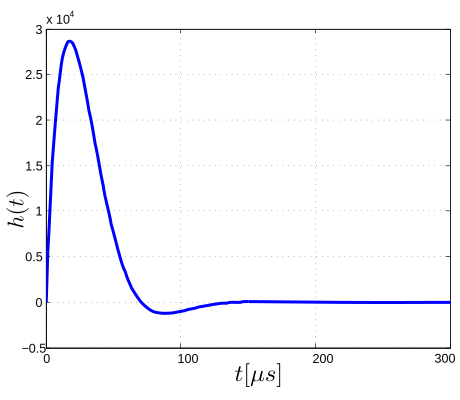
\includegraphics[scale=0.7]{ht.pdf}
    \captionof{figure}{Impulzní charakteristika}
    \label{SAS:fig_ImpChar}
    \par}
  
  Z hlediska analýzy obvodů v kmitočtové oblasti je výhodné sestavovat obvodové rovnice (metodami
  uzlových napětí a smyčkových proudů) přímo v operátorovém tvaru. Kirchhoffovy zákony pro
  uzavřenou smyčku a proudu do uzlu pak mají tvar $$\sum_{k=1}^{n}U_k(p) = 0, \qquad
  \sum_{k=1}^{n}I_k(p) = 0.$$ Metodou uzlových napětí pro zapojení na obr. \ref{SAS:fig_RLC}
  obdržíme rovnice
  \begin{align}
    \frac{U_3(p)-U_1(p)}{R}+\frac{U_3(p)-U_2(p)}{pL} &=  0 \\
    pCU_2(p) + \frac{U_2(p)-U_3(p)}{pL}              &=  0 
  \end{align}
  Na rozdíl od \ref{SAS:eq_RLC_basic_rces} jde o algebraické rovnice, ze kterých eliminací
  uzlového napětí $U_3(p)$ vyplývá přenosová funkce \ref{sas:eq_Hp_RLC} $$H(p) =
  \frac{U_2(p)}{U_1(p)}=\frac{1}{LC}\frac{1}{p^2+p\frac{R}{L}+\frac{1}{LC}}$$
  
   {\centering
    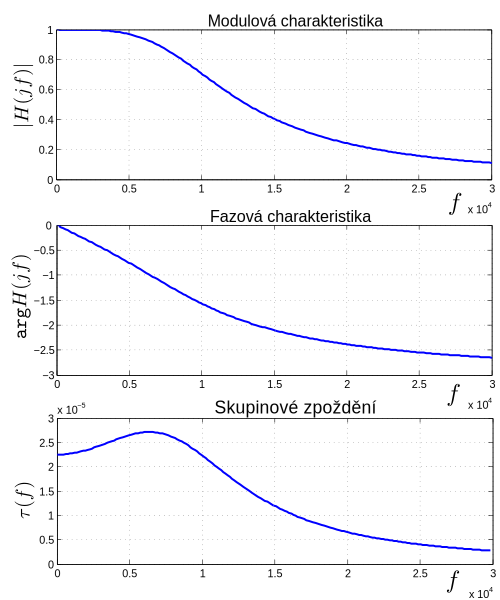
\includegraphics[width=0.7\linewidth]{cir_RLC_response_H_PHA_GD.pdf}
    \captionof{figure}{Modulová, fázová charakteristika a skupinové zpoždění filtru}
    \label{SAS:fig_ex01_RLC}
    \par}    
  
  Dosazením za $p=j\omega$ lze z přenosové funkce vyjádřit modulovou charakteristiku $H(j\omega)$
  a fázovou charakteristiku $\Phi(\omega)= \texttt{arg} H(j\omega)$. Skupinové zpoždění vyplývá
  ze vztahu \ref{SAS:eq_skupinove_zpozdeni}. Modulová, fázová charakteristika a skupinové
  zpoždění jsou na obr. \ref{SAS:fig_ex01_RLC}.
  
  Filtr má maximálně plochou modulovou charakteristiku přenosu. Mezní kmitočet propustného pásma
  je $f_p = 10 kHz$, při kterém je $|H(j\omega_p)|= 0.707$. Tato hodnota odpovídá poklesu
  modulové charakteristiky o $3 dB$.
  
  %---------------------------------------------------------------
  \lstinputlisting{../src/TKY/matlab/SAS_exam_03_Hp.m}
  \begin{lstlisting}[caption=TKY\_exam\_03\_Hp.m]
  \end{lstlisting}
  %--------------------------------------------------------------     
\end{example} 